\begin{center}
	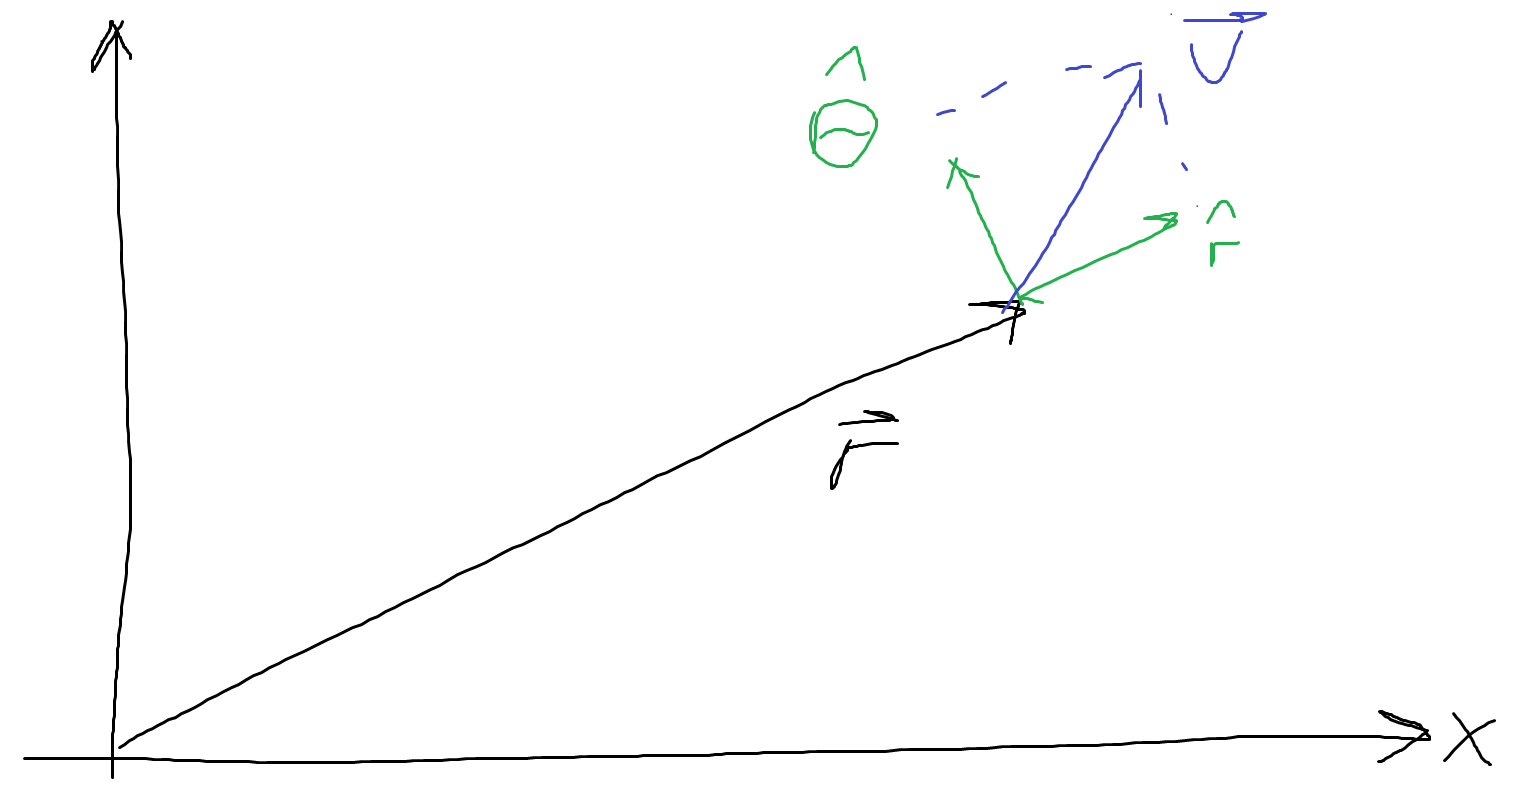
\includegraphics[scale=0.2]{./lect4/pic1.png}
\end{center}
\begin{align*}\left(\mbox{\FiveStarOpen\FiveStarOpen}\right) & \dot{\vec{r}} = \frac{dr}{dt} \cdot \hat{r} + r\frac{d\hat{r}}{dt} =  \frac{dr}{dt} \cdot \hat{r} + r \frac{(d \theta)}{d t}\cdot \hat{\theta}\end{align*}


\paragraph{Acceleration} $$\vec{a} = \frac{d\vec{v}}{dt} = \frac{d}{dt}\left( \frac{d\vec{r}}{dt} \right) = \frac{d^2\vec{r}}{dt^2}$$

Cartesian:

$$\vec{a} = \frac{d^2x}{dt^2}\hat{x} + \frac{d^2y}{dt^2}\hat{y} + \frac{d^2z}{dt^2}\hat{z}$$

Polar:

\begin{align*}\vec{a} = \frac{d\vec{v}}{dt} \stackrel{\mbox{\FiveStarOpen\FiveStarOpen}}{=} \frac{d}{dt}\left( \frac{dr}{dt}\hat{r} + r\frac{d\theta}{dt}\hat{\theta} \right) = \frac{d^2r}{dt^2}\hat{r} + \frac{dr}{dt} \cdot \frac{d\hat{r}}{dt} + \frac{dr}{dt}\cdot\frac{d\theta}{dt}\hat{\theta}  + r\frac{d^2\theta}{dt^2}\hat{\theta}  + r\frac{d\theta}{dt}\frac{d\hat{\theta}}{dt} =\\=
\frac{d^2r}{dt^2}\hat{r} + \frac{dr}{dt} \cdot \frac{d \theta }{d t} \cdot \hat{\theta}+ \frac{dr}{dt}\cdot\frac{d\theta}{dt}\hat{\theta}  + r\frac{d^2\theta}{dt^2}\hat{\theta}  - r\frac{d\theta}{dt}^2 \hat{r} = \left[ \frac{d^2 r}{dt^2} - r \frac{d\theta}{dt}^2\right]\hat{r} + \left[ 2 \frac{dr}{dt}\frac{d\theta}{dt} + r\frac{d^2\theta}{dt^2} \right]\hat{\theta}\end{align*}

$$\vec{a} = \left[ \frac{d^2r}{dt^2} - r\left( \frac{d\theta}{dt} \right)^2 \right]\hat{r} + \frac{1}{r} \left[ \frac{d}{dt}\left( r^2 \frac{d\theta}{dt} \right) \right]\hat{\theta}$$


\subsection{Check common cases}
\begin{enumerate}
	\item $\frac{{d\theta}}{dt} = 0 $
	
	$$	\vec{a} = \left[ \frac{d^2r}{dt^2} - 0 \right]\hat{r} + \frac{1}{r} \left[ \frac{d}{dt}\left( 0 \right) \right]\hat{\theta} =  \frac{d^2\vec{r}}{dt^2}$$
	\item $r = const $ and $\frac{d\theta}{dt} = \omega$
	
	$$\vec{a} = \left[ 0 - r\left( \frac{d\theta}{dt} \right)^2 \right]\hat{r} + \frac{1}{r} \left[ 0 \right]\hat{\theta} = -r\omega^2\hat{r}$$
\end{enumerate}

\paragraph{Circle motion} $r = const$ and $\frac{d\theta}{dt} = \omega = const$

\begin{center}
	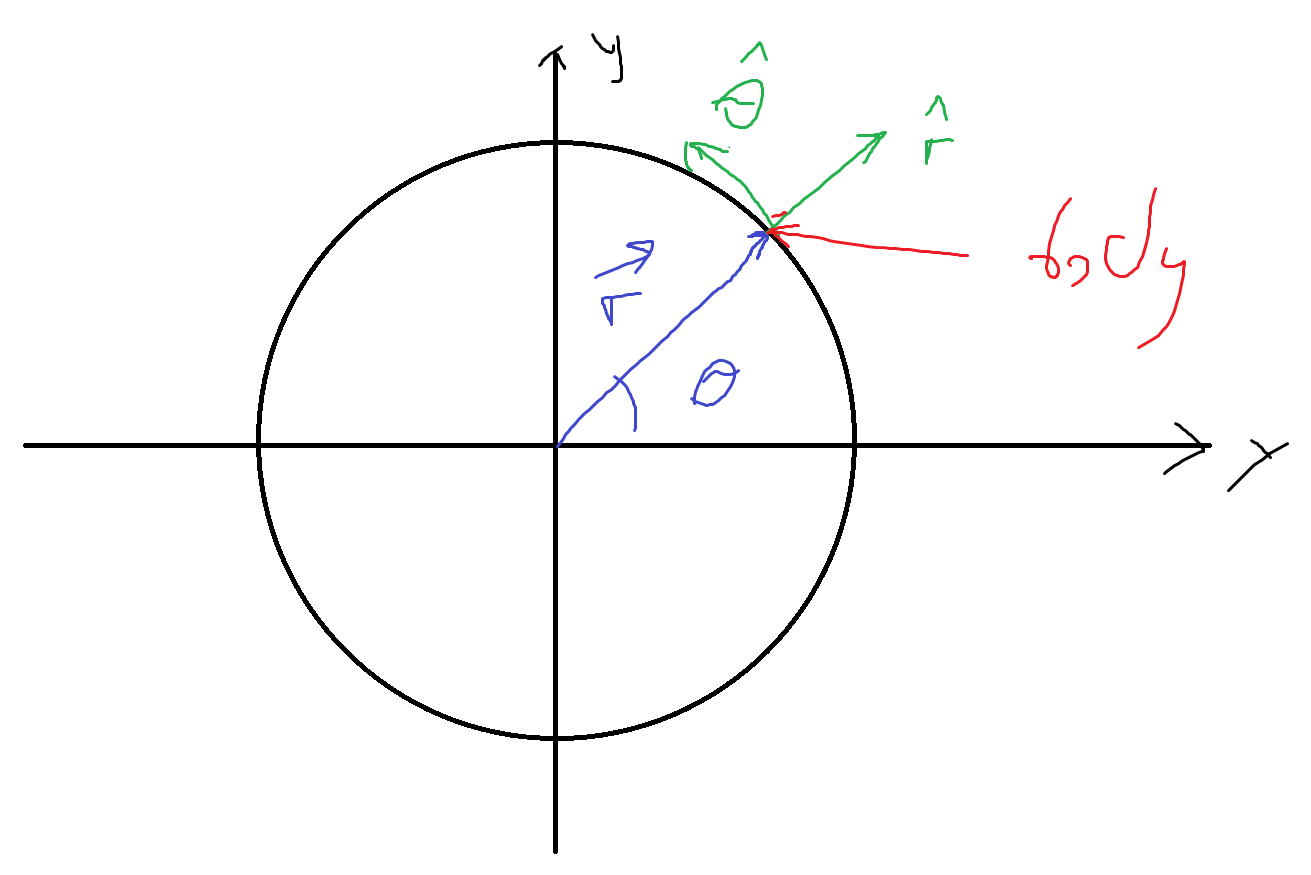
\includegraphics[width=\linewidth]{./lect4/pic2.png}
\end{center}

$$\vec{v} = r \frac{d\theta}{dt}\hat{\theta} = r\omega\hat{\theta}$$

Let at $t=0$ $\theta=0$. At different time $t$ exist following connections:

$$\theta = \omega t$$

In Cartesian:

$$\vec{r} = x(t) \hat{x} + y(t) \hat{t} = r\cos\theta \hat{x} + r\sin\theta\hat{y}$$

Then:

$$\vec{r} = r \cos\left( \omega t\right) \hat{x} + r \sin \left( \omega t \right) \hat{y} $$

$$\vec{v} = \underbrace{- \omega r \sin \left( \omega t \right)}_{v_x} \hat{x} + \underbrace{\omega r \cos \left( \omega t \right)}_{v_y} \hat{y} $$

$$ v = \sqrt{v_x^2 + v_y^2} = \omega r $$

$$\vec{a} = - \omega^2r \cos \left( \omega t \right) \hat{x}  - \omega^2 r \sin \left( \omega t \right) \hat{y} = \omega^2 r \left[ \cos \left( \omega t \right) \hat{x} + \sin \left( \omega t \right) \hat{y} \right] = \omega^2 r \hat{r}$$


\section{Newton laws}
Isaak Newton(1643-1727)
\subsection{First law of Newton}
A body at rest or moving with constant velocity will keep its velocity unless there is force acting on body
\subsection{Second law of Newton}
The rate of change of momentum of a body, is directly proportional to the force applied.

$$\vec{F} = \frac{d\vec{p}}{dt} = \frac{d}{dt}\left(m\vec{v}\right) = \frac{dm}{dt}\vec{v} + m\frac{d\vec{v}}{dt}$$ 

If mass is constant:

$$\vec{F} = m\vec{a}$$

$m$ is inertial mass or mass.
\subsection{Third law of Newton}
When 2 bodies interact, the force first body exerts  on the second is equal in magnitude and opposite in direction to force second body exerts on the first.
\paragraph{Notes}
\begin{enumerate}
	\item Two forces are exerted on different bodies
	\item This law is connected to conservation of momentum
	\item Wrong in special relativity
\end{enumerate}

\paragraph{Example}

$$m\vec{a} = m\frac{d\vec{v}}{dt} = m \frac{d^2r}{dt^2} = m \ddot{\vec{r}}$$

If force is zero:

$$m\frac{d\vec{v}}{dt} = 0 $$

$$\vec{v} = \vec{v}_0 =const $$

$$\frac{d\vec{r}}{dt} = \vec{v}_0 $$

$$d\vec{r} = \vec{v}_0 dt$$

Find integral:

$$\int_{\vec{r}_{beg}}^{\vec{r}_{end}} d\vec{r} = \int_{t_{end}}^{t_{beg}} \vec{v} dt$$

$$\bigg[ \vec{r} \bigg]_{\vec{r}_0}^{\vec{r}} = \bigg[ \vec{v}_0 t \bigg]_{\vec{t}_0}^{\vec{t}}$$

$$\vec{r} - \vec{r}_0 = \vec{v}_t - \vec{v}_0t$$

$$\vec{r}(t) = \vec{r}_0 + \vec{v}_0\left( t-t_0 \right)$$

\subsection{Movement}
Movement is an equation describing position of body changing with a time
\paragraph{Second law} $$\vec{F} = m \vec{a} = m \ddot{\vec{r}} = m \frac{d^2 \vec{r}}{d t^2}$$ It's differential equation.

\paragraph{Example} Constant acceleration on surface Earth.

$$\vec{F} = - mg \hat{y}$$

Using second law for a constant mass:

$$\underbrace{m}_{\parbox{2cm}{\scriptsize  \centering gravitational\\ mass}} \frac{d^2 \vec{r}}{dt^2} = -\underbrace{m}_{\parbox{1cm}{\scriptsize  \centering inertial\\ mass}}g \hat{y}$$

$$-g\hat{y} = \hat{x} \frac{d^2x}{dt^2} + \hat{y}\frac{d^2y}{dt^2}$$

$$\frac{dx^2}{dt^2} = 0$$

$$\frac{d^2y}{dt^2}=-g$$

Solution is:

$$x_0 = x_0 + v_{x0}t$$

$$y= y_0 + v_{y0}t +- \frac{1}{2}gt^2$$

$$v_y = v_{y0} -gt$$